% ============================================================
\chapter{Variables, Types, and Basic Operations}
\label{ch:variables}
% ============================================================

\section{Variables: Labeled Boxes}

\begin{intuition}
A \textbf{variable}\index{variable} is like a labeled box in which you store a value. The label (the name) lets you retrieve the content at any time.
\end{intuition}

\begin{center}
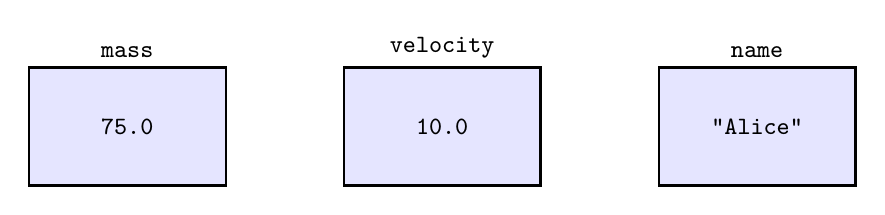
\begin{tikzpicture}
  \foreach \name/\val/\x in {mass/75.0/0, velocity/10.0/4, name/{"Alice"}/8} {
    \draw[thick, fill=blue!10] (\x,0) rectangle (\x+2.5,1.5);
    \node[font=\small\ttfamily] at (\x+1.25,0.75) {\val};
    \node[font=\small\ttfamily, above] at (\x+1.25,1.5) {\name};
  }
\end{tikzpicture}
\end{center}

\begin{codeblock}[title=\textbf{Python --- Creating variables}]
\begin{minted}{python}
# Create variables
mass = 75.0          # decimal number (float)
age = 20             # integer (int)
name = "Alice"       # string (str)
is_student = True    # boolean (bool)

print(f"Name: {name}, Age: {age}")
print(f"Mass: {mass} kg")
print(f"Student: {is_student}")
\end{minted}
\end{codeblock}

\begin{codeoutput}
\begin{verbatim}
Name: Alice, Age: 20
Mass: 75.0 kg
Student: True
\end{verbatim}
\end{codeoutput}

\begin{warning}
In Python, you do not ``declare'' a variable's type. Python figures it out automatically. This is called \textbf{dynamic typing}\index{dynamic typing}.
\end{warning}

\section{Data Types}

\begin{definition}[Fundamental types]\index{types}
Python has four fundamental types:
\begin{itemize}
\item \py{int} --- integer: \py{42}, \py{-7}, \py{0}
\item \py{float} --- decimal: \py{3.14}, \py{-0.5}, \py{6.022e23}
\item \py{str} --- string: \py{"Hello"}, \py{'xyz'}
\item \py{bool} --- boolean: \py{True}, \py{False}
\end{itemize}
\end{definition}

\begin{codeblock}[title=\textbf{Python --- Checking types}]
\begin{minted}{python}
x = 42
y = 3.14
z = "physics"
b = True

print(type(x))   # <class 'int'>
print(type(y))   # <class 'float'>
print(type(z))   # <class 'str'>
print(type(b))   # <class 'bool'>
\end{minted}
\end{codeblock}

\begin{codeoutput}
\begin{verbatim}
<class 'int'>
<class 'float'>
<class 'str'>
<class 'bool'>
\end{verbatim}
\end{codeoutput}

\section{Scientific Notation}

\begin{codeblock}[title=\textbf{Python --- Scientific notation}]
\begin{minted}{python}
# Physical constants in scientific notation
c = 2.998e8        # speed of light (m/s)
h = 6.626e-34      # Planck's constant (J·s)
Na = 6.022e23      # Avogadro's number (mol⁻¹)
G = 6.674e-11      # gravitational constant

print(f"c  = {c}")
print(f"h  = {h}")
print(f"Na = {Na}")
print(f"G  = {G}")
\end{minted}
\end{codeblock}

\begin{codeoutput}
\begin{verbatim}
c  = 299800000.0
h  = 6.626e-34
Na = 6.022e+23
G  = 6.674e-11
\end{verbatim}
\end{codeoutput}

\section{Type Conversion}

\begin{codeblock}[title=\textbf{Python --- Conversions}]
\begin{minted}{python}
# int -> float
x = float(42)
print(x, type(x))        # 42.0 <class 'float'>

# float -> int (truncates!)
y = int(3.99)
print(y, type(y))        # 3 <class 'int'>

# str -> int or float
temperature = int("25")
pi_approx = float("3.14")
print(temperature, pi_approx)

# Number -> str
message = "The answer is " + str(42)
print(message)
\end{minted}
\end{codeblock}

\begin{codeoutput}
\begin{verbatim}
42.0 <class 'float'>
3 <class 'int'>
25 3.14
The answer is 42
\end{verbatim}
\end{codeoutput}

\section{String Operations}

\begin{codeblock}[title=\textbf{Python --- Strings}]
\begin{minted}{python}
first = "Marie"
last = "Curie"

# Concatenation
full_name = first + " " + last
print(full_name)

# Repetition
print("-" * 30)

# Length
print(f"Length: {len(full_name)}")

# Index access (starts at 0!)
print(f"First letter: {full_name[0]}")
print(f"Last letter: {full_name[-1]}")

# Useful methods
print(full_name.upper())
print(full_name.lower())
print(full_name.replace("Curie", "Sklodowska-Curie"))
\end{minted}
\end{codeblock}

\begin{codeoutput}
\begin{verbatim}
Marie Curie
------------------------------
Length: 11
First letter: M
Last letter: e
MARIE CURIE
marie curie
Marie Sklodowska-Curie
\end{verbatim}
\end{codeoutput}

\begin{center}
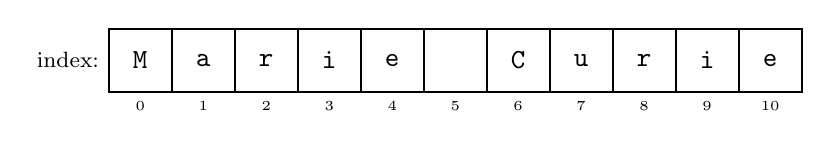
\begin{tikzpicture}
  \foreach \c/\i in {M/0,a/1,r/2,i/3,e/4,{~}/5,C/6,u/7,r/8,i/9,e/10} {
    \draw[thick] (\i*0.8,0) rectangle (\i*0.8+0.8,0.8);
    \node[font=\ttfamily] at (\i*0.8+0.4,0.4) {\c};
    \node[font=\tiny,below] at (\i*0.8+0.4,0) {\i};
  }
  \node[font=\footnotesize,left] at (0,0.4) {index:};
\end{tikzpicture}
\end{center}

\section{f-strings (Formatted Strings)}

\begin{codeblock}[title=\textbf{Python --- f-strings}]
\begin{minted}{python}
element = "Hydrogen"
atomic_mass = 1.008
number = 1

# f-string: insert variables into text
print(f"Element {element} (Z={number}) has mass {atomic_mass} u")

# Number formatting
pi = 3.141592653589793
print(f"pi = {pi:.2f}")      # 2 decimals
print(f"pi = {pi:.6f}")      # 6 decimals
print(f"pi = {pi:.2e}")      # scientific notation

# Alignment
for element, mass in [("H", 1.008), ("C", 12.011), ("O", 15.999)]:
    print(f"{element:<5} {mass:>8.3f} u")
\end{minted}
\end{codeblock}

\begin{codeoutput}
\begin{verbatim}
Element Hydrogen (Z=1) has mass 1.008 u
pi = 3.14
pi = 3.141593
pi = 3.14e+00
H         1.008 u
C        12.011 u
O        15.999 u
\end{verbatim}
\end{codeoutput}

\section{Comparison Operators and Booleans}

\begin{codeblock}[title=\textbf{Python --- Comparisons}]
\begin{minted}{python}
x = 10
print(x > 5)       # True
print(x == 10)      # True (equality)
print(x != 7)       # True (not equal)
print(x >= 15)      # False

# Logical operators
a = True
b = False
print(a and b)      # False
print(a or b)       # True
print(not a)        # False
\end{minted}
\end{codeblock}

\begin{codeoutput}
\begin{verbatim}
True
True
True
False
False
True
False
\end{verbatim}
\end{codeoutput}

\begin{keyformulas}[title=\textbf{Comparison Operators}]
\begin{tabular}{lll}
\toprule
\textbf{Operator} & \textbf{Meaning} & \textbf{Example} \\
\midrule
\py{==} & Equal to & \py{5 == 5} $\to$ \py{True} \\
\py{!=} & Not equal to & \py{5 != 3} $\to$ \py{True} \\
\py{<}, \py{>} & Less than, greater than & \py{3 < 5} $\to$ \py{True} \\
\py{<=}, \py{>=} & Less or equal, greater or equal & \py{5 >= 5} $\to$ \py{True} \\
\py{and} & Logical AND & \py{True and False} $\to$ \py{False} \\
\py{or} & Logical OR & \py{True or False} $\to$ \py{True} \\
\py{not} & Logical NOT & \py{not True} $\to$ \py{False} \\
\bottomrule
\end{tabular}
\end{keyformulas}

\section{User Input}

\begin{codeblock}[title=\textbf{Python --- input}]
\begin{minted}{python}
# input() always returns a string!
# name = input("Your name: ")
# age = int(input("Your age: "))
# print(f"Hello {name}, you are {age} years old.")

# Simulation (for the course)
name = "Alice"
age = 20
print(f"Hello {name}, you are {age} years old.")
\end{minted}
\end{codeblock}

\begin{codeoutput}
\begin{verbatim}
Hello Alice, you are 20 years old.
\end{verbatim}
\end{codeoutput}

\section{Common Pitfalls}

\begin{errmark}
\begin{codeblock}[title=\textbf{Common errors}]
\begin{minted}{python}
# 1. Forgetting quotes for strings
# name = Alice        # NameError: name 'Alice' is not defined
name = "Alice"        # Correct

# 2. Confusing = (assignment) and == (comparison)
x = 5                # assigns 5 to x
# x == 5             # compares x to 5, returns True

# 3. Integer division surprise
print(7 / 2)         # 3.5 (Python 3, ok)
print(7 // 2)        # 3 (integer division!)

# 4. Concatenating number and string
# print("I am " + 20 + " years old")  # TypeError
print("I am " + str(20) + " years old")  # OK
print(f"I am {20} years old")            # Even better
\end{minted}
\end{codeblock}
\end{errmark}

\section{Mini-Project: Atom Identity Card}

\begin{projet}
Create a program that displays an atom's identity card.

\begin{codeblock}[title=\textbf{Python}]
\begin{minted}{python}
# Identity card: Carbon
element = "Carbon"
symbol = "C"
atomic_number = 6
atomic_mass = 12.011  # u
electronegativity = 2.55  # Pauling

print("=" * 35)
print(f"  IDENTITY CARD: {element}")
print("=" * 35)
print(f"  Symbol            : {symbol}")
print(f"  Atomic number     : {atomic_number}")
print(f"  Atomic mass       : {atomic_mass} u")
print(f"  Electronegativity : {electronegativity}")
print(f"  Number of protons : {atomic_number}")
print(f"  Number of electrons: {atomic_number}")
print("=" * 35)
\end{minted}
\end{codeblock}

\begin{codeoutput}
\begin{verbatim}
===================================
  IDENTITY CARD: Carbon
===================================
  Symbol            : C
  Atomic number     : 6
  Atomic mass       : 12.011 u
  Electronegativity : 2.55
  Number of protons : 6
  Number of electrons: 6
===================================
\end{verbatim}
\end{codeoutput}
\end{projet}

\section{Exercises}

\begin{exercise}[$\star$ --- Guided]
Create variables for the Boltzmann constant ($k_B = 1.381 \times 10^{-23}$~J/K) and temperature $T = 300$~K. Compute thermal energy $E = k_B T$ and display the result.
\end{exercise}

\begin{exercise}[$\star$ --- Guided]
Create a variable \py{radius = 6371} (Earth's radius in km). Compute and display the circumference ($C = 2\pi r$) and surface area ($S = 4\pi r^2$) of Earth.
\end{exercise}

\begin{exercise}[$\star\star$ --- Independent]
Write a program that asks the user for a distance in kilometers and converts it to miles (1~km $= 0.621$~miles), meters, and centimeters.
\end{exercise}

\begin{exercise}[$\star\star$ --- Independent]
Create a program that computes BMI (Body Mass Index): $\text{BMI} = \frac{\text{mass (kg)}}{\text{height (m)}^2}$. Display the result with 1 decimal place.
\end{exercise}

\begin{exercise}[$\star\star\star$ --- Scientific Challenge]
The photon energy formula is $E = hf = hc/\lambda$. Compute the energy of a red photon ($\lambda = 700$~nm) and a blue photon ($\lambda = 450$~nm). Express results in joules and electron-volts ($1$~eV $= 1.602 \times 10^{-19}$~J).
\end{exercise}

\begin{keyformulas}[title=\textbf{Chapter Summary}]
\begin{itemize}
\item A variable stores a value: \py{x = 42}.
\item Types: \py{int}, \py{float}, \py{str}, \py{bool}.
\item \py{type(x)} gives the type, \py{int()}/\py{float()}/\py{str()} convert.
\item Scientific notation: \py{6.022e23} = $6.022 \times 10^{23}$.
\item f-strings: \py{f"pi = \{pi:.2f\}"} for formatting.
\item Comparison operators: \py{==}, \py{!=}, \py{<}, \py{>}, \py{and}, \py{or}.
\end{itemize}
\end{keyformulas}
